\newpage
\section{Conception et mise en œuvre}
\label{sec:impl}

\subsection{Architecture globale du logiciel}
\paragraph{} L'architecture du projet suit le modèle MVC (Modèle-Vue-Contrôleur) :

\begin{itemize}
\item \textbf{Modèle (engine.data)} : Classes Card, Deck, Player, GameStats
\item \textbf{Contrôleur (engine.process)} : Classes Game, Combination, BotPlayer
\item \textbf{Vue (gui)} : Classes MainGUI, MenuGUI, OptionGUI, EndGameGUI
\end{itemize}

\begin{figure}[h!]
\centering
%\includegraphics[width=12cm]{images/architecture.png}
\caption{Architecture du logiciel}
\label{fig:architecture}
\end{figure}

\subsection{Classes de données (engine.data)}
\paragraph{}
\begin{itemize}
\item \textbf{Card} : Représente une carte avec sa valeur et sa couleur. Implémente equals() et hashCode().
\item \textbf{Deck} : Gère le paquet de 54 cartes, mélange (shuffle) et pioche (draw).
\item \textbf{Player} : Gère la main du joueur, la pioche et la pose de combinaisons.
\item \textbf{CombinationType} : Énumération des types (SIMPLE, DOUBLE, SERIES, BOMB, DOUBLE\_JOKER, INVALID).
\item \textbf{GameStats} : Enregistre les statistiques et calcule les scores.
\end{itemize}

\subsection{Traitements (engine.process)}
\paragraph{}
\begin{itemize}
\item \textbf{Combination} : Détection automatique du type avec determineType(), comparaison avec canBeat().
\item \textbf{Game} : Logique principale (gestion des tours, pioche, reset, recyclage).
\item \textbf{BotPlayer} : Classe abstraite avec stratégies différentes.
\item \textbf{EasyBot} : Joue aléatoirement, 30\% de chance de passer.
\item \textbf{MediumBot} : Évite les bombes, joue les combinaisons faibles.
\item \textbf{HardBot} : Stratégique, privilégie les combinaisons fortes.
\end{itemize}

\begin{figure}[h!]
\centering
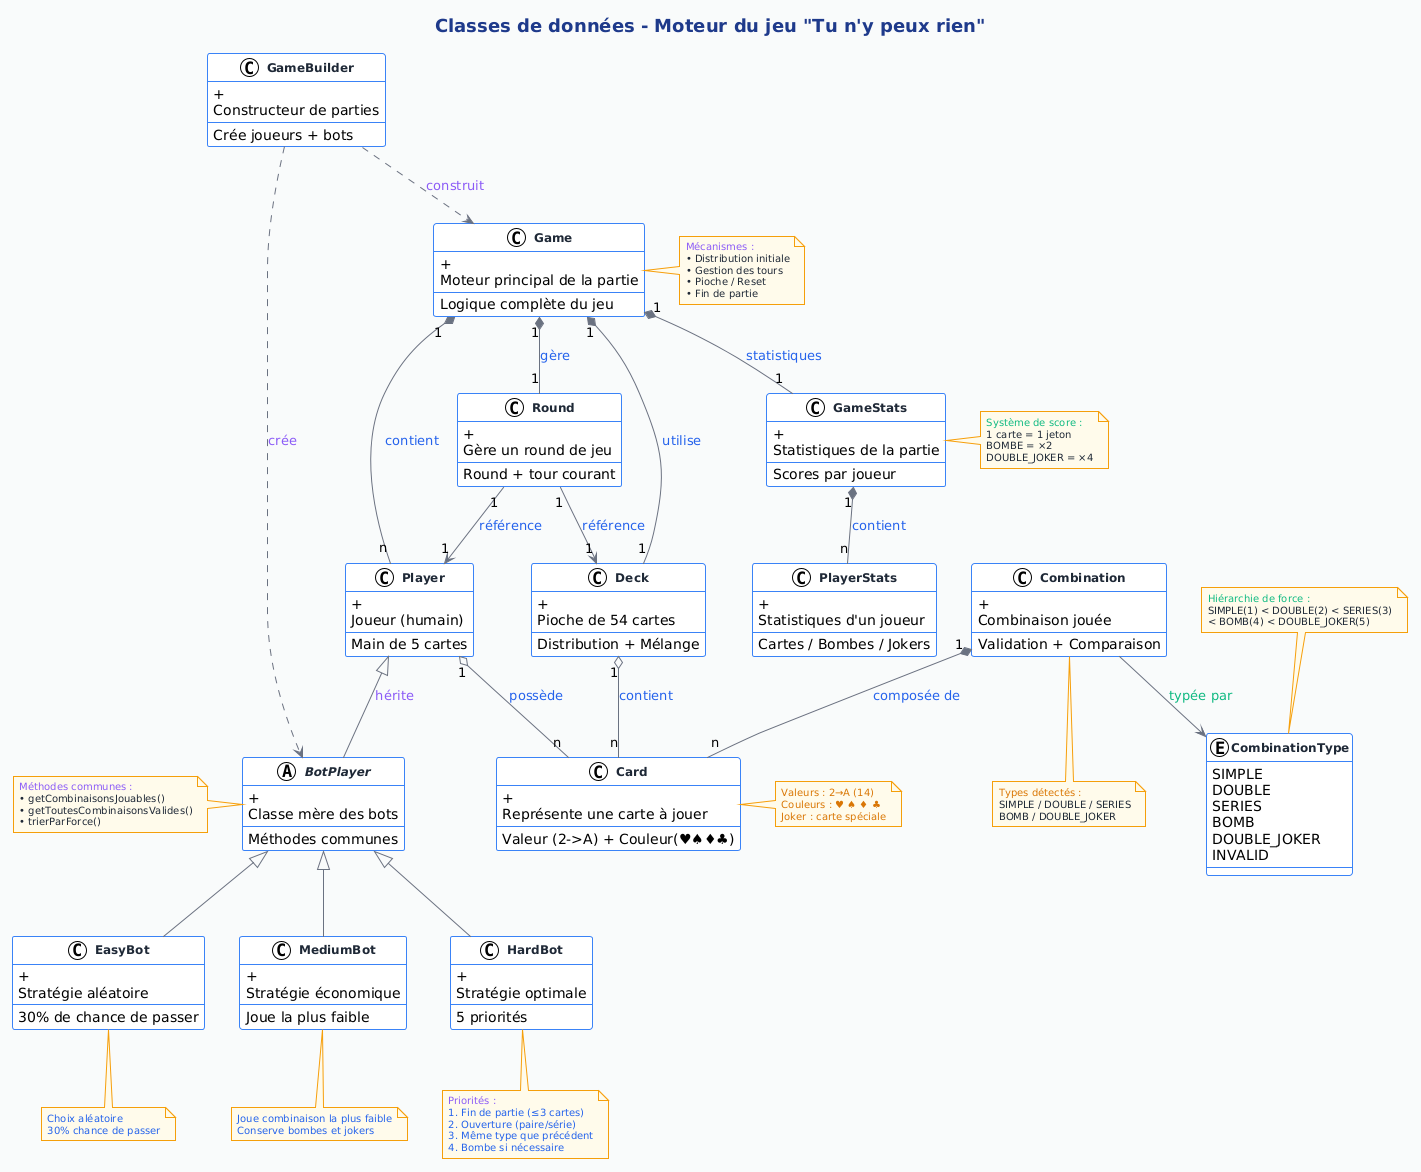
\includegraphics[width=14cm]{images/diagramme_classes.png}
\caption{Diagramme de classes UML}
\label{fig:uml}
\end{figure}

\subsection{IHM Graphique (gui)}
\paragraph{} L'interface est organisée en trois sous-dossiers :

\begin{itemize}
\item \textbf{screens/} : Écrans complets (MainGUI, MenuGUI, OptionGUI, EndGameGUI)
\item \textbf{panels/} : Composants réutilisables (CardPanel, BotsPanel, DeckPanel, GameInfoBar, GameLogPanel)
\item \textbf{utils/} : Utilitaires (GameStyle, CardPaintStrategy, MusicPlayer)
\end{itemize}

\subsection{Patterns de conception utilisés}
\paragraph{}
\begin{itemize}
\item \textbf{Héritage} : BotPlayer → EasyBot, MediumBot, HardBot
\item \textbf{Factory} : GameBuilder.createBot()
\item \textbf{MVC implicite} : Séparation data/process/gui
\item \textbf{Stratégie} : Comportements différents des bots
\item \textbf{Singleton implicite} : GameStyle.isFullscreen
\end{itemize}
